% 由固定来源示意图按 a=1（或 t=1）重绘；保留两抛物线、公共交点 O/A 与 A 点切线的拓扑关系。
\begin{center}
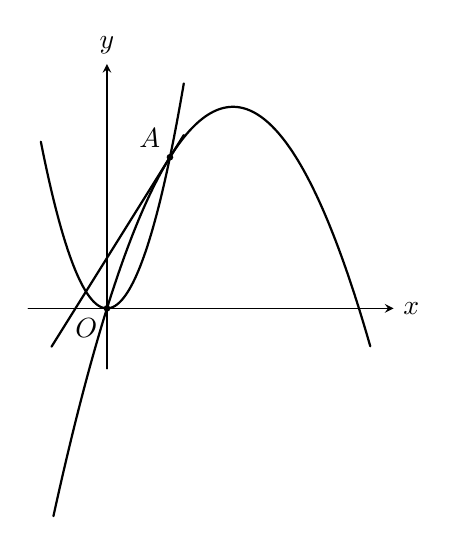
\begin{tikzpicture}[x=0.8cm,y=0.64cm,>=stealth,line cap=round,line join=round]
  \draw[->] (-1.25,0)--(4.55,0) node[right] {$x$};
  \draw[->] (0,-1.2)--(0,4.85) node[above] {$y$};
  \draw[thick,domain=-1.05:1.22,samples=80] plot (\x,{3*\x*\x});
  \draw[thick,domain=-0.85:4.18,samples=120] plot (\x,{-\x*\x+4*\x});
  \draw[thick] (-0.88,-0.76)--(1.22,3.44);
  \fill (0,0) circle (1.2pt);
  \fill (1,3) circle (1.2pt);
  \node[below left] at (0,0) {$O$};
  \node[above left] at (1,3) {$A$};
\end{tikzpicture}
\end{center}
